\documentclass[11pt]{article}

\usepackage[margin=1.1in]{geometry}
\usepackage{graphicx}
\usepackage{booktabs}
\usepackage{amsmath}
\usepackage{microtype}
\usepackage[hidelinks]{hyperref}
\usepackage{natbib}

\title{Argmax Decoding Causes Liquidity Failure\\
in a Market of Language-Model Traders}

\author{%
  D. Holzricher\\
  \texttt{dholzric@gmail.com}
}

\date{September 2026}

\begin{document}
\maketitle

\begin{abstract}
We populate a continuous double auction with traders whose decisions are made
by a typed language model that returns a probability distribution over actions,
and vary only how that distribution is consumed. Taking the model's modal
action---the default in virtually every deployment---makes the market stop
trading after shocks: following a positive shock, the market clears in
$65.6\%$ of periods against $91.3\%$ after a negative shock, a gap of
$25.8$ percentage points (95\% CI $[17.3, 34.2]$, $t=6.37$, $n=20$
preregistered). Sampling from the same distribution reduces the gap to
$3.1$ points. Two algorithmic baselines that are symmetric by construction show
no gap. The mechanism is direct and observable: $100\%$ of non-trading periods
under modal decoding had one side of the order book entirely empty, against
$3.4\%$ for the zero-intelligence baseline. Because every trader conditions on
the same public signal, a deterministic policy makes them act identically, and
a market of unanimous buyers has no counterparty. The effect decomposes into
two parts: unanimity sets its magnitude, while a standing directional bias in
the arm's order flow determines which shock it strikes.

We test this mechanism with a preregistered prediction it could have failed:
if unanimity is the cause, the effect must vanish as the market grows. It does,
from $37.0$ points at four traders to $4.2$ at thirty-two
($-0.112$ per doubling, $t=-6.91$). A companion prediction---that sampling
would show no such decay---was falsified: sampling herds too, seven times more
weakly, on the same curve. We therefore report a single mechanism whose
strength is set by how sharply the decode rule collapses the model's
distribution, rather than two regimes.

Separately, we find that ordinary domain wording induces a $25$-point
asymmetry in the model's stated conviction between buying and selling at equal
mispricing, which vanishes under mirror-image phrasing. A preregistered test
found this does \emph{not} move pricing error, and we report that null.

All experiments were preregistered, including the two hypotheses that failed.
\end{abstract}

\section{Introduction}

A language model asked to choose among actions returns, in principle, a
distribution. Almost every deployment discards it and takes the mode. For a
single decision this is correct: the mode is the most likely action. This paper
asks what happens when many agents driven by the same model make related
decisions at the same time.

The answer, in a market, is that the market stops. Modal decoding makes agents
conditioning on shared information act identically. In a setting that requires
counterparties, unanimity is not consensus; it is the absence of trade. We
measure this in a continuous double auction, isolate the mechanism, and confirm
it with a prediction that could have failed and did not.

Our contributions:

\begin{enumerate}
\item \textbf{A liquidity failure caused by decoding, not by reasoning.} The
  model's modal action is \emph{correct} on both sides at every mispricing we
  tested. Nothing about its judgement is wrong. The failure is entirely in the
  aggregation of correct decisions.
\item \textbf{A directly observed mechanism, in two parts.} We instrument both
  sides of the order book and show that under modal decoding, non-trading
  periods lack a counterparty essentially always, while for symmetric baselines
  they do not. Unanimity sets the magnitude; a standing directional bias in
  order flow sets which shock it strikes. Our own first account used only the
  former and is corrected in Section~\ref{par:two}.
\item \textbf{A falsifiable size-scaling test.} The mechanism implies the
  effect must decay with market size at a rate set by the agreement rate. We
  registered this before running it; it held.
\item \textbf{A prompt-sensitivity result, and a null.} Domain-idiomatic
  wording induces a large conviction asymmetry invisible to anyone reading only
  the modal action. A preregistered test found it does not move pricing error.
\end{enumerate}

We emphasise the failures. Three preregistered predictions in this project were
wrong, and each is reported: the original mechanism (Section~\ref{sec:wording}),
the sampling-amplification prediction, and the claim that sampling would show no
size decay (Section~\ref{sec:size}). The result that survived did so against
tests designed to kill it.

\section{Related work}

\paragraph{Market design and baselines.} The experimental market tradition
begins with \citet{smith1962}. Our lower baseline is the zero-intelligence
trader of \citet{gode1993}, whose result---that budget-constrained random
traders achieve high allocative efficiency---makes a random arm a genuine floor
rather than a strawman, and motivates the value clamp that prevents any arm in
our design from knowingly trading at a loss.

\paragraph{LLM agents in simulated markets.} \citet{lopezlira2025} builds a
simulated stock market with a persistent order book in which heterogeneous LLM
agents submit structured decisions, and reports that agents adhere consistently
to assigned strategies while the market reproduces price discovery, bubbles and
underreaction. That work also notes that prompts can generate correlated
behaviours affecting market stability, which is the phenomenon we isolate and
measure here.

\paragraph{Correlation as systemic risk.} Closest to our result is
\citet{ross2026}, who argue that shared training and architecture make more
capable models behave more similarly, creating a non-diversifiable risk floor,
and who test this with LLM traders of varying capability in an agent-based
market. They find correlated behaviour that \emph{increases} with capability,
and that it becomes a liability when agents share a misinformation
environment.

Our contribution is complementary and, we think, orthogonal in a useful way.
They vary the model and attribute correlation to properties of the model---its
training, its architecture, its capability. We hold the model \emph{fixed} and
vary only how its output distribution is consumed. The correlation we measure
is therefore not a property of the model at all but of a deployment choice,
and it is one a practitioner controls directly: our argmax and sampling arms
issue identical requests and read identical responses, differing only in a
single line of client code. Where \citet{ross2026} identify a risk floor set by
model similarity, we show a large component of realised correlation sitting
above that floor, removable without changing models.

\paragraph{Herding and cascades.} The classical account of correlated action is
the informational cascade of \citet{bikhchandani1992}, in which an agent
rationally ignores private information after observing enough predecessors.
Our mechanism is deliberately simpler and should not be confused with it.
Agents in our market do not observe one another's decisions and draw no
inference from them; they condition on a common public signal and a
deterministic policy maps that signal to the same action. There is no learning,
no sequence, and no inference---only a degenerate policy. The resulting
unanimity looks like herding and has the same market consequence, but it
arises without any of the cascade machinery, which is why it can be switched
off at the decoder.

\paragraph{Decoding and diversity.} That greedy decoding collapses output
diversity is long established in text generation: \citet{holtzman2020} show
that maximisation-based decoding yields repetitive, degenerate text and
introduce nucleus sampling as a remedy. The quality--diversity tension is
well understood \emph{within} a single generation. We report a consequence one
level up: when many agents share a decoder, the diversity that sampling
preserves is not a stylistic property of one output but the raw material a
market needs to clear. Sampling is individually worse and collectively
necessary.

\paragraph{Confidence and calibration.} \citet{kadavath2022} study whether
language models can predict the correctness of their own answers, and
subsequent work has documented systematic overconfidence in verbalised
confidence. Our Experiment~\ref{sec:wording} touches this literature from an
unusual angle: the model we use returns a probability distribution natively
rather than a verbalised estimate, and we find that ordinary domain wording
shifts that distribution by 25 points without changing the selected option.
Any calibration measurement taken over such a model inherits whatever asymmetry
the question's phrasing introduced.

\paragraph{What we could not find.} We did not find prior work isolating the
decode rule as a cause of market-level liquidity failure, nor a preregistered
size-scaling test of a herding mechanism in an LLM-populated market. We would
welcome pointers; this survey was conducted by the authors and is not
exhaustive.

\section{The instrument}

\subsection{Market}

A continuous double auction in one abstract good. Prices are integer ticks;
matching is price-then-time priority; an incoming order executes at the resting
order's price. A trader's resting orders are withdrawn at the top of its turn,
so each trader has at most one live order. Submitting on one side cancels the
trader's resting orders on the other, preventing wash trades without leaving a
crossed book.

Accounts are conserved by construction. Each trade moves cash from buyer to
seller and inventory from seller to buyer, one for one. Short sales and
borrowing are disallowed, and every order is pre-checked against uncommitted
cash or uncommitted inventory. A property test submits 20{,}000 random orders
and asserts after every one that total cash and total units are exactly their
endowed values, that no account is negative, that no trader has committed more
than it holds, and that the book is never crossed.

Order size is fixed at one unit, so aggressiveness is the only lever an arm
has; position sizing is a second channel and is deliberately disabled.

\subsection{Fundamental and information}

The fundamental $F_t$ is piecewise constant. For the size and liquidity
experiments we use a \emph{matched-jump} process: jumps are evenly spaced, of
identical magnitude, strictly alternating in direction, and even in number, so
that every up window is paired with a down window of the same size between the
same two price levels. This makes the up-versus-down comparison within-run and
matched, which matters: under a random-jump process the per-run noise on this
statistic has standard deviation $0.74$, large enough that a single seed of the
symmetric baseline returned a spurious $-0.82$ gap.

Each trader's private value is $F_t + \varepsilon_{i,t}$ with
$\varepsilon \sim \mathcal{N}(0, 5)$, redrawn each period. All experiments here
use full information; the delayed and noisy signal treatments are implemented
but not reported.

\subsection{The decision contract}

Code owns matching, budgets, order sizes and prices. An agent answers three
typed questions and nothing else: direction (\texttt{buy}/\texttt{sell}/%
\texttt{pass}), urgency on a five-level scale, and whether the signal is
already reflected in the book. A code-owned rule maps urgency to an integer
tick, anchored on the book and hard-clamped at the agent's own private value.

That clamp is load-bearing. \emph{An agent cannot express a losing price},
because it never expresses a price. A 20{,}000-case property test asserts that
no quote is ever on the wrong side of the quoting agent's value. Consequently
every effect we report is about direction and timing, never about arithmetic.

The question wording is frozen and hash-locked; a test fails if any instruction
or criterion changes. This is the defence against unrecorded prompt iteration.

\subsection{Arms}

All four arms emit the same object, including a distribution over
$\{\texttt{buy}, \texttt{sell}, \texttt{pass}\}$, which makes them comparable.

\begin{itemize}
\item \textbf{ZI}: random direction and urgency, fixed policy distribution,
  value-clamped so it never knowingly trades at a loss.
\item \textbf{NBR}: logit best-response over the same urgency grid, scored by
  expected surplus times a fill probability. Exactly symmetric between sides by
  construction; a buy at mispricing $+x$ and a sell at $-x$ receive identical
  probability.
\item \textbf{Jev-argmax}: the model's modal action.
\item \textbf{Jev-sample}: a draw from the model's distribution.
\end{itemize}

The two model arms read one response, so for a given observation they are one
API call and differ only in the decode rule.

\section{The model and its measurement properties}

The model is a commercially available typed-decision model that returns, for a
multiple-choice question, a selected option together with a probability over
all options. Three properties affect measurement and are reported because they
constrain what can be claimed.

\paragraph{Non-determinism.} Identical requests return different answers. Four
repetitions of one request returned urgency scores of $2.84$, $2.79$, $2.82$
and $2.74$ and buy probabilities of $0.98$, $0.99$, $0.99$, $0.99$. There is no
seed parameter. Run-to-run noise is roughly $\pm 0.05$ on a $0$--$4$ urgency
scale and $\pm 0.01$ on probabilities. \emph{Reproducibility therefore requires
the response archive, not merely the code}: a rerun without it does not
reproduce. All 110{,}805 responses are retained and every reported figure is
regenerable from them.

\paragraph{Quantisation.} Probabilities are returned to two decimal places, so
three-option distributions routinely sum to $0.99$ or $1.01$. We accept and
renormalise within tolerance.

\paragraph{Undocumented failure modes.} The published status codes are
incomplete; the service returns bare \texttt{5xx} from its edge under load. A
client written to the documentation alone will treat these as fatal.

\section{Experiment 1: wording, conviction, and a null}
\label{sec:wording}

\subsection{Domain wording induces a conviction asymmetry}

Our first criteria were written in ordinary domain language: \emph{buy} as ``the
good is underpriced\ldots you want to acquire a unit'', \emph{sell} as ``the
good is overpriced\ldots you want to dispose of a unit''. At equal absolute
mispricing the model placed $0.988$ on the profitable side when buying was
correct and $0.738$ when selling was correct, a gap of $0.250$, with the
missing mass on \texttt{pass}.

The gap survives a second price level ($+0.225$), reversing the option order
($+0.235$), and renaming the options neutrally ($+0.185$). It does not survive
rewriting the two criteria as exact structural mirrors---``value is
\emph{above} the price'' versus ``\emph{below} the price''---under neutral
instructions, where the gap is $+0.005$ (Figure~\ref{fig:wording}).

\begin{figure}[t]
\centering
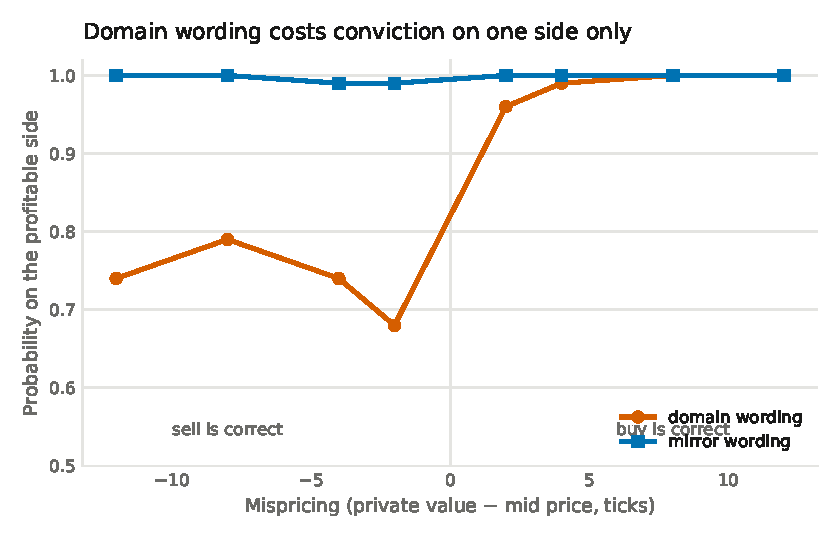
\includegraphics[width=0.78\textwidth]{../figures/fig2_wording.pdf}
\caption{Probability the model places on the profitable side, against
mispricing, under the two wordings. The model is symmetric when asked
symmetrically. The effect is $25\times$ the model's own run-to-run noise.}
\label{fig:wording}
\end{figure}

Two points matter for practice. First, the modal action is \emph{correct on
both sides at every point tested}: a practitioner reading only the selected
option sees nothing wrong. Second, the wording that induces the skew is the
natural one; symmetry had to be engineered deliberately.

\subsection{It does not move pricing error}

We predicted this skew would slow price discovery after negative shocks. A
four-seed exploratory run supported it ($+0.63$, four of four seeds positive,
Holm $p=0.061$). We registered the test and ran it on twenty fresh seeds. It
failed: $-0.184$, 95\% CI $[-0.479, +0.111]$, seven of nineteen seeds positive,
one-sided $p=0.897$. The confirmatory interval excludes the exploratory
estimate. With $\mathrm{SE}=0.140$ the run had ample power to detect the
exploratory effect, so this is evidence of absence.

We report it as such. Wording skews what the model says; it does not, in this
market, change what prices do.

\section{Experiment 2: liquidity failure under modal decoding}
\label{sec:liquidity}

The null above was correct for the question it asked, and the question was
wrong. Root mean squared pricing error is defined only over periods in which
trade occurred, and so discards exactly the periods where the effect lives. In
one run, modal decoding produced zero trades in all three up-jump windows and
full trading in all three down-jump windows---270 trades in the run, none in
the 45 periods after a positive shock.

We therefore registered a new outcome, defined for every period:
$\mathrm{traded}(d)$, the share of the fifteen periods after a jump of
direction $d$ in which at least one trade occurred.

\begin{table}[t]
\centering
\begin{tabular}{lrrr}
\toprule
& \multicolumn{2}{c}{Traded share} & \\
\cmidrule(lr){2-3}
Arm & after up & after down & Gap \\
\midrule
Jev-argmax   & $66.6\%$ & $93.8\%$ & $+25.8$ \\
Jev-sample   & $93.0\%$ & $93.9\%$ & $+3.1$ \\
ZI           & $77.3\%$ & $75.0\%$ & $-0.4$ \\
NBR          & $99.8\%$ & $99.3\%$ & $+1.0$ \\
\bottomrule
\end{tabular}
\caption{Preregistered confirmatory test, twenty fresh seeds. D1: the
Jev-argmax gap exceeds zero, $t=6.37$, eighteen of twenty seeds positive.
D2: it exceeds the Jev-sample gap by $22.7$ points, $t=6.01$. Both
Holm-significant.}
\label{tab:liquidity}
\end{table}

\paragraph{Mechanism, observed.} We instrument resting depth on both sides at
the close of every period, which separates two failures: \emph{no counterparty}
(one side empty) and \emph{no crossing} (both sides present, prices do not
meet). Table~\ref{tab:silence} classifies every silent post-shock period.

\begin{table}[t]
\centering
\begin{tabular}{llrrr}
\toprule
Arm & Shock & No seller & No buyer & Both sides, no cross \
\midrule
Jev-argmax & up   & $\mathbf{100.0\%}$ & $0.0\%$ & $0.0\%$ \
           & down & $96.2\%$ & $0.0\%$ & $3.8\%$ \
Jev-sample & up   & $71.4\%$ & $4.3\%$ & $24.3\%$ \
           & down & $57.1\%$ & $7.1\%$ & $35.7\%$ \
ZI         & up   & $0.9\%$  & $2.8\%$ & $96.3\%$ \
           & down & $2.3\%$  & $1.8\%$ & $95.9\%$ \
NBR        & up   & $8.3\%$  & $0.0\%$ & $91.7\%$ \
           & down & $0.0\%$  & $0.0\%$ & $100.0\%$ \
\bottomrule
\end{tabular}
\caption{Why each silent post-shock period was silent, twenty seeds. Under
modal decoding the market is missing a counterparty essentially always; the
symmetric baselines fall silent the ordinary way, with both sides quoting and
prices failing to meet.}
\label{tab:silence}
\end{table}

The failure is unambiguous and one-sided: the market runs out of
\emph{sellers}. It is never short of buyers in any arm.

\paragraph{Two components, not one.}
\label{par:two}
Unanimity alone does not account for the direction of the effect, and we report
this because our own account of it was initially wrong. Measured directly, the
agreement rate is \emph{higher} after down shocks ($96\%$) than up shocks
($92\%$), while the halt is far worse after up shocks. A pure unanimity story
predicts the opposite ordering.

Order flow resolves it (Table~\ref{tab:flow}). The modal arm carries a standing
buy bias, and the two shocks interact with it differently. After an up shock
the bias compounds with the shock and order flow becomes overwhelmingly
one-sided. After a down shock---where every trader's value lies below the
prevailing price and selling is plainly indicated---the arm still issues
\emph{more buys than sells}. It never reaches a sell majority. The bias and the
shock roughly cancel, flow stays mixed, and the market continues to clear.

\begin{table}[t]
\centering
\begin{tabular}{llrrr}
\toprule
Arm & Shock & Buy & Sell & Pass \
\midrule
Jev-argmax & up   & $65.9\%$ & $28.2\%$ & $5.8\%$ \
           & down & $\mathbf{48.8\%}$ & $\mathbf{42.3\%}$ & $8.8\%$ \
Jev-sample & up   & $44.3\%$ & $34.9\%$ & $20.8\%$ \
           & down & $41.2\%$ & $39.0\%$ & $19.8\%$ \
ZI         & up   & $46.2\%$ & $44.1\%$ & $9.8\%$ \
           & down & $44.8\%$ & $45.9\%$ & $9.3\%$ \
NBR        & up   & $51.6\%$ & $48.4\%$ & $0.0\%$ \
           & down & $47.9\%$ & $52.1\%$ & $0.0\%$ \
\bottomrule
\end{tabular}
\caption{Order flow in the fifteen periods after a shock. Both algorithmic
baselines respond to shock direction symmetrically. The modal arm does not: it
issues more buys than sells even after a down shock, which is why the down-side
halt is mild and the up-side halt severe.}
\label{tab:flow}
\end{table}

So the effect decomposes. \textbf{Unanimity} sets its magnitude and produces
the size-scaling of Section~\ref{sec:size}: with more traders, the chance that
every one of them agrees falls, and the halt fades. \textbf{A directional bias}
sets which shock it strikes, by determining whether the bias reinforces or
offsets the shock. The sampling arm exhibits the same bias in muted form
($41.2\%$ versus $39.0\%$ after a down shock), consistent with the falsified E2
of Section~\ref{sec:size}: sampling dilutes correlation rather than removing
it.

\paragraph{A control that does not quite hold.} NBR returns $+1.0$ points
($t=3.33$), small but distinguishable from zero, indicating a slight genuine
structural tilt in the market. It is $1/26$ of the effect under test, ZI is
clean ($-0.4$, $t=-0.22$), and it does not survive the per-size controls of
Section~\ref{sec:size}. We report it because the registration required controls
to sit on zero and this one does not.

\section{Experiment 3: the mechanism, tested where it could fail}
\label{sec:size}

If the market halts because every trader reaches the same conclusion, the
effect must depend on the number of traders. With agreement rate $p$ measured
independently at $0.92$, the probability that all $N$ agree is approximately
$p^N$, which falls from $0.72$ at $N=4$ to $0.07$ at $N=32$. We registered two
predictions before running: that the argmax gap would decay with $N$ (E1), and
that the sampling gap would not (E2).

\begin{figure}[t]
\centering
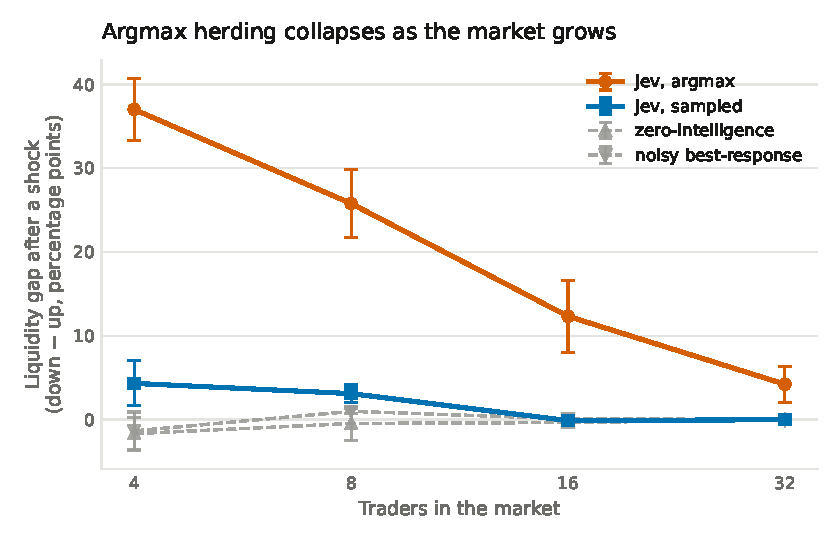
\includegraphics[width=0.78\textwidth]{../figures/fig1_market_size.pdf}
\caption{The liquidity gap against market size, twenty seeds per point, bars
are standard errors. At $N=32$ both symmetric baselines trade in $100\%$ of
periods with a zero gap, so there is no structural floor and the residual
$4.2$ points is attributable to the arm.}
\label{fig:size}
\end{figure}

\paragraph{E1 confirmed.} The gap falls from $37.0$ points at $N=4$ to $4.2$ at
$N=32$; slope $-0.112$ per doubling, $t=-6.91$. It is robust to dropping the
$N=4$ point, which we flagged in advance as floor-constrained because the
symmetric baselines themselves trade in only $33\%$ of periods there
($-0.108$, $t=-4.21$).

\paragraph{E2 falsified.} We predicted sampling would show no decay. It shows
$-0.016$ per doubling, $t=-2.53$. The available rescue---attributing it to the
floor-constrained $N=4$ point---fails: dropping that point makes the decay
\emph{more} significant ($t=-3.53$).

The corrected account is better than the prediction. Sampling herds as well,
seven times more weakly, on the same curve. At a buy probability of $0.99$,
most sampled traders still choose to buy; sampling does not abolish correlation
but dilutes it. There is one mechanism, whose strength is set by how sharply
the decode rule collapses the distribution, rather than two regimes.

\section{Discussion}

The practical claim is narrow and, we think, general in shape: \emph{the best
way to use one model is not the best way to use many of them}. Modal decoding
is individually optimal and collectively degenerate whenever agents share
information and require counterparties or diversity. Sampling is individually
worse---it deliberately takes a less likely action some of the time---and here
it was the difference between a market that cleared and one that did not.

The failure is not a reasoning failure. The model's modal action was correct on
both sides at every mispricing tested. Nothing in its judgement was wrong; the
loss occurred in aggregation. Evaluation of a single agent's decisions cannot
detect this, which is what makes it worth reporting.

\section{Limitations}

\paragraph{The origin of the directional bias.} Section~\ref{par:two}
establishes \emph{that} the modal arm carries a standing buy bias, and that
this bias determines which shock the halt strikes. It does not establish
\emph{why} the bias exists. Both symmetric baselines are balanced at every
market size, so it is not an artefact of the market's construction, but we
cannot presently attribute it to the model, to the task framing, or to the
state representation.

\paragraph{One model.} All results are for a single typed-decision model. We
have no evidence about others, and cannot say whether the agreement rate that
drives the mechanism is characteristic or idiosyncratic.

\paragraph{Provenance of the probabilities.} We treat the returned
probabilities as the model's beliefs. We have asked the vendor whether they are
calibrated posterior mass or post-processed, and have no answer. If the latter,
Experiment~1 is a statement about a serving stack rather than a model.

\paragraph{Full information only.} Every trader observes $F_t$ exactly, which
maximises the correlation the mechanism exploits. The delayed and noisy
treatments are implemented but unreported, and would plausibly weaken the
effect.

\paragraph{Scale.} Markets of four to thirty-two traders over 160 periods. The
extrapolation to larger markets is the fitted decay, not a measurement.

\section{Reproducibility}

Because the model is non-deterministic and has no seed, code alone does not
reproduce these numbers. Every response is archived---110{,}805 of them---and
the analysis can be replayed against the archive with live calls disabled, in
which case a cache miss raises rather than silently contacting the API. Total
spend was approximately \$3.30 across roughly 95{,}000 live calls.

The preregistrations, including the falsified hypotheses and the reasons the
outcome measure changed between Experiments~1 and~2, are in the repository with
their commit timestamps.

\bibliographystyle{plainnat}
\begin{thebibliography}{9}
\bibitem[Gode and Sunder(1993)]{gode1993}
D.~K. Gode and S.~Sunder.
\newblock Allocative efficiency of markets with zero-intelligence traders:
  Market as a partial substitute for individual rationality.
\newblock \emph{Journal of Political Economy}, 101(1):119--137, 1993.

\bibitem[Smith(1962)]{smith1962}
V.~L. Smith.
\newblock An experimental study of competitive market behavior.
\newblock \emph{Journal of Political Economy}, 70(2):111--137, 1962.

\bibitem[Bikhchandani et~al.(1992)]{bikhchandani1992}
S.~Bikhchandani, D.~Hirshleifer, and I.~Welch.
\newblock A theory of fads, fashion, custom, and cultural change as
  informational cascades.
\newblock \emph{Journal of Political Economy}, 100(5):992--1026, 1992.

\bibitem[Holtzman et~al.(2020)]{holtzman2020}
A.~Holtzman, J.~Buys, L.~Du, M.~Forbes, and Y.~Choi.
\newblock The curious case of neural text degeneration.
\newblock In \emph{International Conference on Learning Representations}, 2020.
\newblock arXiv:1904.09751.

\bibitem[Kadavath et~al.(2022)]{kadavath2022}
S.~Kadavath et~al.
\newblock Language models (mostly) know what they know.
\newblock arXiv:2207.05221, 2022.

\bibitem[Lopez-Lira(2025)]{lopezlira2025}
A.~Lopez-Lira.
\newblock Can large language models trade? Testing financial theories with LLM
  agents in market simulations.
\newblock arXiv:2504.10789, 2025.

\bibitem[Ross et~al.(2026)]{ross2026}
J.~Ross, E.~So, Z.~De~Simone, C.~Pozniak, and A.~W. Lo.
\newblock Why better models can create riskier systems: Evidence from LLM
  agents in financial markets.
\newblock arXiv:2609.04373, 2026.
\end{thebibliography}

\end{document}
